\documentclass[a4paper]{report}
\title{Development of 1D Compressible Inviscid Flow Solver Code}
\author{Ramkumar}

\usepackage{graphicx}
\usepackage{subfigure}
\usepackage{cleveref}
\usepackage{framed}
\usepackage{listings}
\usepackage{natbib}

\setlength{\headheight}{1cm}
\setlength{\headsep}{1cm}
\setlength{\topmargin}{1mm}
\setlength{\oddsidemargin}{5mm}
\setlength{\evensidemargin}{-3mm}
\setlength{\textwidth}{160mm}
\setlength{\textheight}{225mm}

\begin{document}
	\maketitle
	\newpage
	\tableofcontents
	\listoffigures
	
	\chapter{Development of 1D Compressible Inviscid Flow Solver Code}
	
	\section{Abstract}
	\paragraph*{}
	The development of 1D compressible inviscid flow solver code is done as present work. The code was developed using two methods for computation, Maccormack's technique and RK4 scheme, with Finite Difference as it base. In former method, the $1^{st}$ order temporal discretization and Maccormack's technique used for spacial discretization. Whereas in latter method, Upwind scheme is used for spacial and RK4 scheme is used for temporal discretizations. The Compressible Euler equations are used for computation. The solver was developed using Python 3.6 language. Finally, validation is done by performing error computations and the results were plotted as graph.
	
	\section{Computation Methodology}
	\begin{enumerate}
		\item. Finite Difference Method is used for computation.
		\item  Two solvers are made, one with Maccormack's predictor-corrector technique for $2^{nd}$ order spacial discretization and $1^{st}$ order temporal discretization, whereas other solver is developed with RK4 scheme for temporal and $1^{st}$ order Upwind for spacial discretizations.
		\item  one dimensional, constant cross-section area field is chosen as computational domain. Hence, all the primitive parameters will be same at all nodes at the end of computation.
		\item  for validation purposes, air is taken as fluid medium and respective properties are taken.
		\item The compressible Euler equations are taken as governing equations for computation.
		\item validation is performed by running the solver code for 3 different grids and errors were computed by comparing the velocity field with inlet velocity.
		\item the RMS errors and Error percentages are plotted against grid spaces for validating the solver.		
	\end{enumerate} 

	\newpage	

	\section{Results and Conclusions}
	\begin{figure}[htb!]		
		\subfigure[]{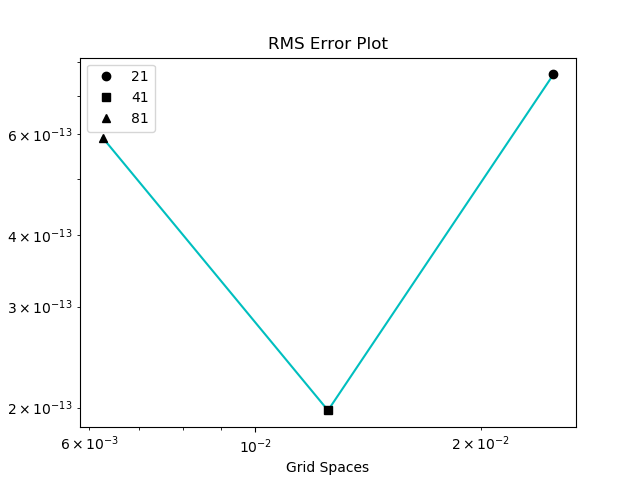
\includegraphics[scale=0.6]{RMSError_M.png}\label{RMS_M}}
		\subfigure[]{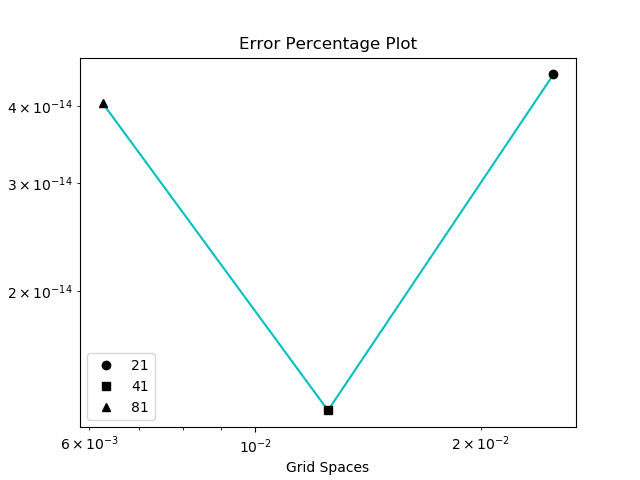
\includegraphics[scale=0.6]{ErrorPercentage_M.png}\label{EP_M}}
		
		\caption{Graphs depicting the variation of \subref{RMS_M} RMS Error with grid spaces \subref{EP_M} Error percentages with grid spaces, for the solver using Maccormack method}
		\label{M_graphs}	
	\end{figure}
	\begin{figure}[htb!]
		\subfigure[]{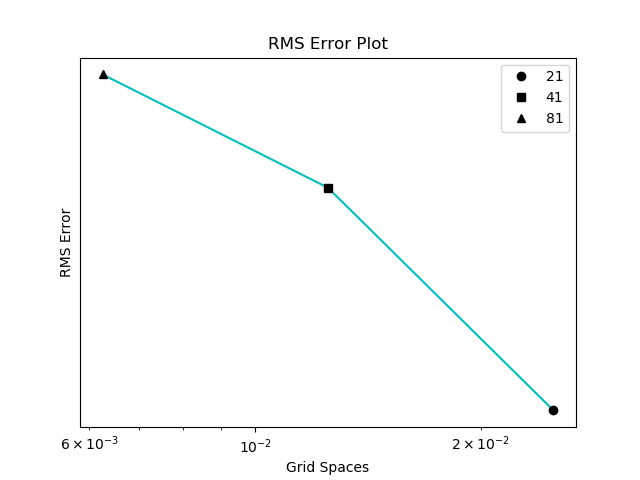
\includegraphics[scale=0.6]{RMSError_R.png}\label{RMS_R}}
		\subfigure[]{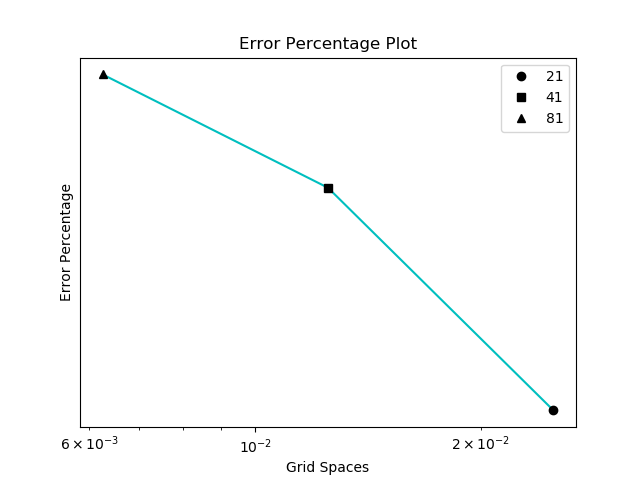
\includegraphics[scale=0.6]{ErrorPercentage_R.png}\label{EP_R}}
		
		\caption{Graphs depicting the variation of \subref{RMS_R} RMS Error with grid spaces \subref{EP_R} Error percentages with grid spaces, for the solver using RK4 method}
		\label{R_graphs}
	\end{figure}
	
	\newpage
	The graphs \cref{M_graphs} and \cref{R_graphs} represent the variation of rms errors and error percentages of solvers using Maccormack and RK4 methods respectively. The rms error and error percentage for Maccormack method are of order $10^{-13}$ and $10^{-14}$ respectively. Similarly for RK4 method, they were of same order. The increase in error with decrease in grid spacing, as seen from the graph, is due to the machine epsilon and linear variation of solution result, i.e. constant velocity throughout the domain. Hence, it can be concluded that the solver is validated and found to be working perfectly. The following are the source codes of the solver.
	
	\section{Source Code: Maccormack Solver}
	the source code of the solver that uses Maccormack method is given below
	\begin{framed}
		\lstset{breaklines=true}
		\lstinputlisting{Mscript.py}
	\end{framed}

	\section{Source Code: RK4 Solver}
	The source code of the solver that uses RK4 Method is given below
	\begin{framed}
		\lstset{breaklines=true}
		\lstinputlisting{Rscript.py}
	\end{framed}

	\renewcommand{\bibname}{References}
	%\bibliographystyle{plain}
	\bibliographystyle{unsrtnat}
	\nocite{*}
	\bibliography{bibliog}
\end{document}
